%\begin{figure}[!htbp]
%    \centering
%    \caption{}
%    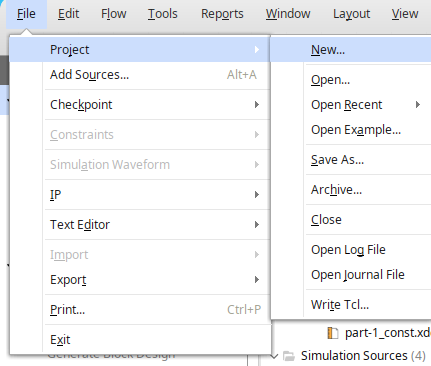
\includegraphics[width=0.5\textwidth]{figure_3_1.png}
%    \label{Figure 3.1}
%\end{figure}\newline

%\begin{center}
%    Truth Table 1: AND Gate Waveform
%    \begin{displaymath}
%    \begin{array}{|c c|c|}
%    In1 & In2 & In1 \land In2\\
%    \hline
%    F & F & F\\
%    F & T & F\\
%    T & F & F\\
%    T & T & T\\
%    \end{array}
%    \end{displaymath}
%\end{center}

\documentclass{article}
\usepackage{graphicx} % Required for inserting images
\usepackage{varwidth}
\usepackage{listings}
\usepackage{xcolor}

\title{Experiment 4 Lab Report \\ \large EEE3342C - 00012}
\author{Yousef Awad}
\date{March 2025}
\setcounter{secnumdepth}{0}

\lstdefinestyle{Verilog}{
  language=Verilog,
  basicstyle=\ttfamily\small,
  keywordstyle=\color{blue}\bfseries,
  commentstyle=\color{gray},
  stringstyle=\color{purple},
  numbers=left,
  numberstyle=\tiny,
  stepnumber=1,
  numbersep=5pt,
  tabsize=2,
  breaklines=true,
  captionpos=b,
  frame=single
}

\begin{document}

\maketitle
\tableofcontents
\newpage

\section{Equipment}
For this experiment a computer running Linux 6.12.13 was used alongside the Xilinx Vivado 2024.2 software, alongside an FPGA board, the BASYS 3 development board. The board specifically only used to ensure the simulation by the Vivado software was accurate in the real world, as well as to verify the simulation software wasn't incorrect.
\section{Objective}
\section{Part 1: Half/Full Adder}
\subsection{Half Adder}
The circuit given for this part was the following:
$$ \neg[(A \land B) \lor \neg (C \lor D)] $$

Of which has the following given schematic:
\begin{figure}[!htbp]
    \centering
    \caption{Schematic for Half Adder}
    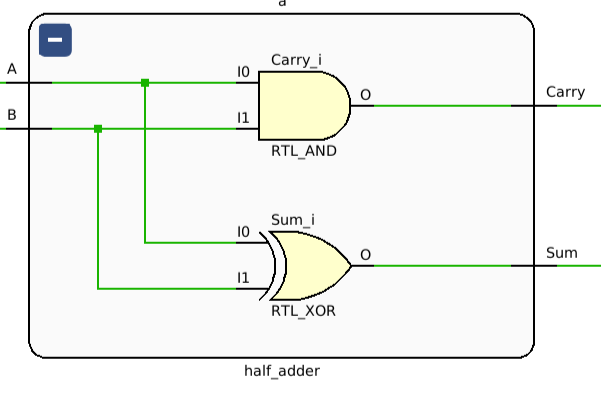
\includegraphics[width=0.5\textwidth]{part-1-half-schem.png}
    \label{Half Adder Schematic}
\end{figure}

And when compiled into a truth table with the inputs of A, B, and an output of Carry, would be the following:
\begin{center}
    Truth Table for Half Adder
    \begin{displaymath}
    \begin{array}{|c c|c c|}
      A & B & Output & Carry\\
    \hline
    F & F & F & F \\
    F & T & T & F \\
    T & F & T & F \\
    T & T & F & T \\
    \end{array}
    \end{displaymath}
\end{center}
\newpage
And when written up in verilog, has the following text:
\begin{lstlisting}[label={label}, style=Verilog]
module half_adder(
      input A, B,
      output Sum, Carry
  );
  
  assign Sum = A ^ B;
  assign Carry = A & B;
  
endmodule
\end{lstlisting}

And when tested, used the following testbench, after reading through part 1 of the experiment manual:
\begin{lstlisting}[label={label}, style=Verilog]
module testbench();
    parameter numin = 2;
    integer i;
    reg[numin - 1:0] count;
    
    reg a, b;
    wire carry, sum;
    
    half_adder UUT(.A(a), .B(b), .Carry(carry), .Sum(sum));

    
    initial begin
        count = 0;
        for ( i = 0; i < 2**numin; i = i + 1 ) begin
            assign a = count[1];
            assign b = count[0];
            
            count = count + 1;
            #10;
        end
    end
    
endmodule
\end{lstlisting}

And, when simulated to confirm the truth table above to be true or false, it gave out the following waveform:
\begin{figure}[!htbp]
    \centering
    \caption{Waveform for the Half-Adder}
    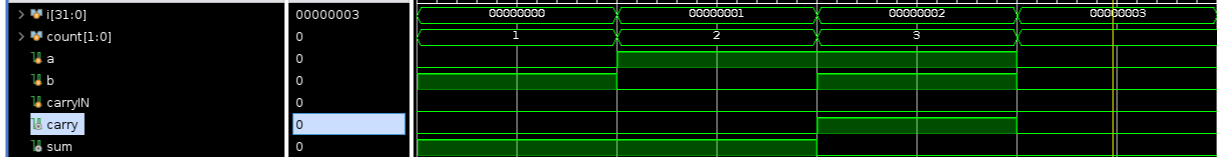
\includegraphics[width=1\textwidth]{part-1-half-waveform.png}
    \label{Figure 2}
\end{figure}
\newpage
Of which perfectly shows that the truth table compiled above for the circuit is accurately shown in the simulation on Vivado. To ensure, even further, I then pushed the bitstream generated onto the BASYS board to manually enter and double check the simulation/truth table proper by flicking every possible combination.

\subsection{Full Adder}
The circuit schematic given for this part was the following:

\begin{figure}[!htbp]
    \centering
    \caption{Schematic for Full Adder}
    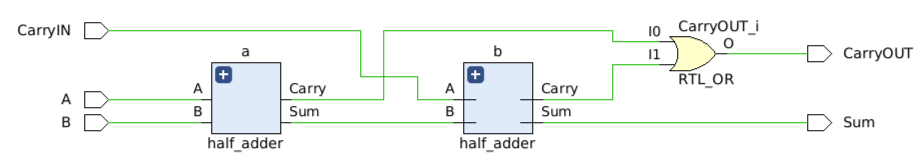
\includegraphics[width=0.5\textwidth]{part-1-full-schem.png}
    \label{Full Adder Schematic}
\end{figure}

And when written up in verilog, has the following text:
\begin{lstlisting}[label={label}, style=Verilog]
module full_adder(
        input A, B, CarryIN,
        output Sum, CarryOUT
    );
    
    wire carry1, carry2, sum1;
    
    half_adder a(.A(A), .B(B), .Carry(carry1), .Sum(sum1));
    half_adder b(.A(CarryIN), .B(sum1), .Sum(Sum), .Carry(carry2));
    
    assign CarryOUT = carry1 | carry2; 
    
endmodule
\end{lstlisting}
\newpage
And when tested, used the following testbench, after reading through part 1 of the experiment manual:
\begin{lstlisting}[label={label}, style=Verilog]
module testbench();
    parameter numin = 2;
    integer i;
    reg[numin - 1:0] count;
    
    reg a, b, carryIN;
    wire carry, sum;
    
    full_adder UUT(.A(a), .B(b), .CarryIN(carryIN), .CarryOUT(carry), .Sum(sum));

    
    initial begin
        count = 0;
        for ( i = 0; i < 2**numin; i = i + 1 ) begin
            assign a = count[1];
            assign b = count[0];
            assign carryIN = 0;
            
            count = count + 1;
            #10;
        end
    end
    
endmodule
\end{lstlisting}

And, when simulated, it gave out the following correct waveform:
\begin{figure}[!htbp]
    \centering
    \caption{Waveform for the Half-Adder}
    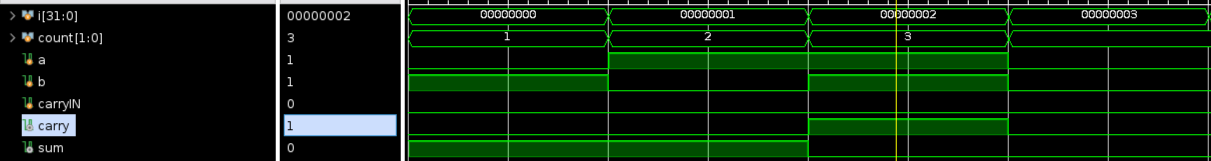
\includegraphics[width=1\textwidth]{part-1-full-waveform.png}
    \label{Figure 2}
\end{figure}

To ensure, even further past the given truth table in lab report, I then pushed the bitstream generated onto the BASYS board to manually enter and double check the simulation proper by flicking every possible combination.
\newpage


\section{Part 2: 8-Bit Ripple Carry Adder}
The schematic was designed as following:
\begin{figure}[!htbp]
    \centering
    \caption{Schematic for 8 Bit Ripple Carry Adder}
    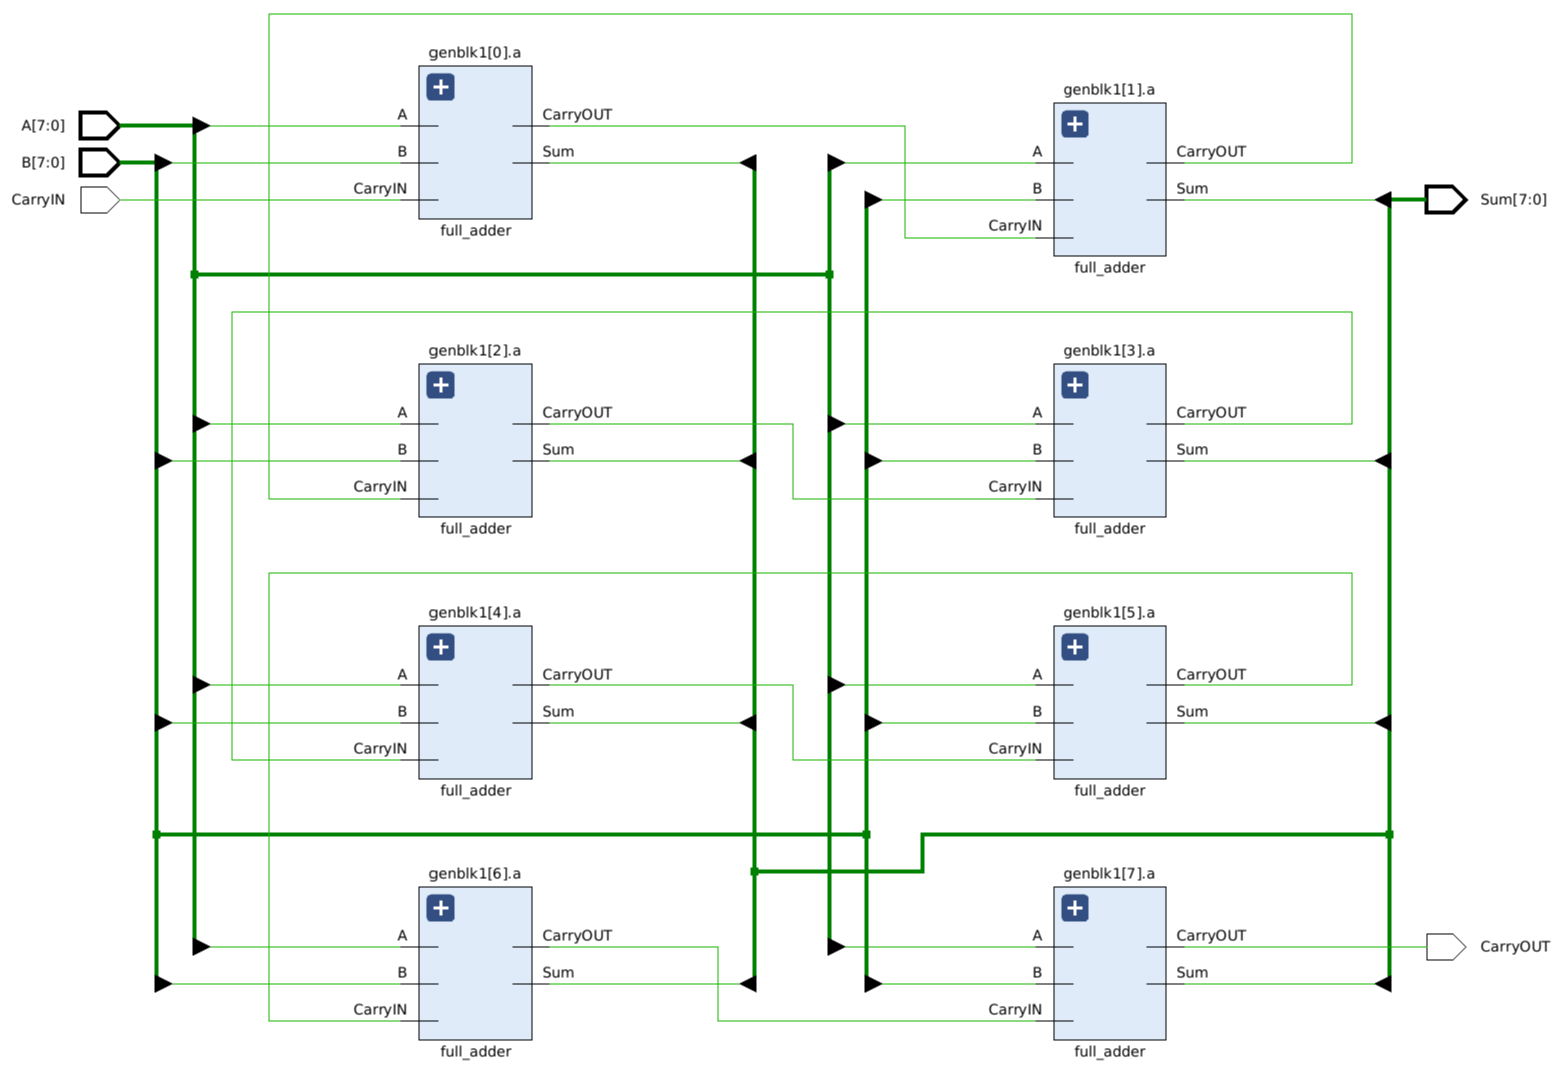
\includegraphics[width=0.5\textwidth]{part-2-schem.png}
    \label{8 Bit Ripple Carry Schematic}
\end{figure}

And when written up in verilog, has the following text:
\begin{lstlisting}[label={label}, style=Verilog]
module eight_bit_ripple_adder(
        input[7:0] A, B, 
        input CarryIN,
        output[7:0] Sum, 
        output CarryOUT
    );
    
    wire[8:0] carry;
    
    assign carry[0] = CarryIN;
    
    genvar i;
    
    generate
        for ( i = 0; i < 8; i = i + 1 ) begin
            full_adder a(.A(A[i]), .B(B[i]), .CarryIN(carry[i]), .CarryOUT(carry[i + 1]), .Sum(Sum[i]));
        end
    endgenerate
    
    assign CarryOUT = carry[8];
    
endmodule
\end{lstlisting}

And when tested, used the following testbench, after reading through part 1 of the experiment manual:
\begin{lstlisting}[label={label}, style=Verilog]
module testbench_part2();
    parameter numin = 8;
    
    reg[numin - 1:0] a, b;
    reg carryIN;
    wire[numin - 1:0] sum;
    wire carryOUT;
    
    eight_bit_ripple_adder UUT(.A(a), .B(b), .CarryIN(carryIN), .CarryOUT(carryOUT), .Sum(sum));
    
    initial begin
        assign a = 8'b11001011;
        assign b = 8'b10101010;
        assign carryIN = 0;
        #10;
        assign carryIN = 1;
        #10
        assign a = 0;
        assign b = 0;
        assign carryIN = 0;
    end
    
endmodule
\end{lstlisting}

And, when simulated to confirm the addition of 170 and 203 (assuming it is unsigned) above to be 0x75 Carry 1 as it overflows and switches sign, it gave out the following waveform:
\begin{figure}[!htbp]
    \centering
    \caption{Waveform for Addition of 0x170 and 0x203}
    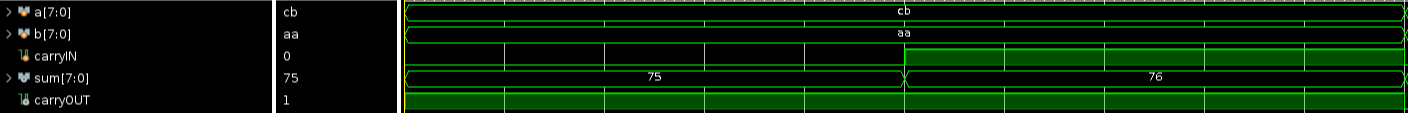
\includegraphics[width=1\textwidth]{part-2-waveform.png}
    \label{Waveform for Addition of 170 and 203}
\end{figure}

Of which perfectly shows the correct result to be 0x75 or 0x76 of which is in binary either 01001011 or 01001100 and in decimal is 117, depending on the carry in value with a carry out of 1 meaning it overflowed.
\newpage


\section{Part 3: Carry Look-Ahead Adder}
The schematic was designed as following:
\begin{figure}[!htbp]
    \centering
    \caption{Schematic for 8 Bit Carry Look-Ahead Adder}
    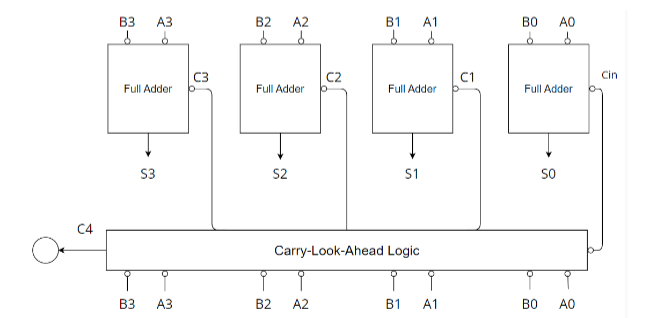
\includegraphics[width=0.5\textwidth]{part-3-schem.png}
    \label{8 Bit Carry Look-Ahead Adder}
\end{figure}

And when written up in verilog, has the following text:
\begin{lstlisting}[label={label}, style=Verilog]
module eight_bit_carry_look_adder( // part 3
    input[7:0] Num1, Num2,
    input CarryIN,
    output[7:0] Sum,
    output CarryOUT
  );
  // why use carry look ahead adders?
  // this gets rid of the propogation delay and therefore is "faster", of which adds in parallel instead of sequentially.
  // this, however, uses a lot more gates to be used and is therefore more area intensive.
  wire[7:0] carryGenerate, carryPropagate, carryTemp;
  genvar i; // temporary variable i
  
  // logic for carry look adders
  assign carryGenerate = Num1 & Num2;
  assign carryPropagate = Num1 ^ Num2;

  assign carryTemp[0] = CarryIN;
  generate
    for ( i = 1; i < 8; i = i + 1) begin
      assign carryTemp[i] = carryGenerate[i - 1] | (carryPropagate[i - 1] & carryTemp[i - 1]);
    end
  endgenerate

  // addition logic proper
  generate
    full_adder a(.A(Num1[0]), .B(Num2[0]), .CarryIN(CarryIN), .CarryOUT(), .Sum(Sum[0]));
    for (i = 1; i < 8; i = i + 1) begin
      full_adder a(.A(Num1[i]), .B(Num2[i]), .CarryIN(carryTemp[i]), .CarryOUT(), .Sum(Sum[i]));
    end
  endgenerate
  
  assign CarryOUT = carryTemp[7];

endmodule
\end{lstlisting}

And when tested, used the following testbench:
\begin{lstlisting}[label={label}, style=Verilog]
module testbench_part3();
  reg [7:0] Num1, Num2;
  reg CarryIN;

  wire[7:0] Sum;
  wire CarryOUT;

  eight_bit_carry_look_adder instance_1(.Num1(Num1), .Num2(Num2), .CarryIN(CarryIN), .CarryOUT(CarryOUT), .Sum(Sum));

  initial begin

    Num1 = 8'b11001011; 
    Num2 = 8'b10101010; 
    CarryIN = 0;
    #10;

  end
endmodule
\end{lstlisting}

And, when simulated to confirm the addition of 11001011 + 10101010 (assuming it is unsigned), it gave out the following waveform:
\begin{figure}[!htbp]
    \centering
    \caption{Waveform Addition CLA}
    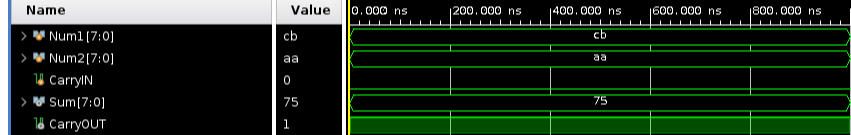
\includegraphics[width=1\textwidth]{part-3-waveform.png}
    \label{Waveform Part 3 A}
\end{figure}

Of which perfectly shows the correct result to be when compared to the addition for the Ripple Carry Adder waveform below: 

\begin{figure}[!htbp]
    \centering
    \caption{Waveform Addition RCA}
    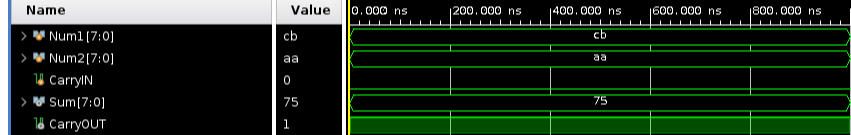
\includegraphics[width=1\textwidth]{part-3-waveform.png}
    \label{Waveform Part 3 B}
\end{figure}
\newpage
And, since both waveforms are the exact same, means that the verilog code proper is, in effect, also the same, at least results wise. Area and latency wise, they are different.
\newpage



\section{Part 4: 32-bit Adder and Subtractor}
The schematic was designed as following:
\begin{figure}[!htbp]
    \centering
    \caption{Schematic for 32 Bit Adder/Subtractor}
    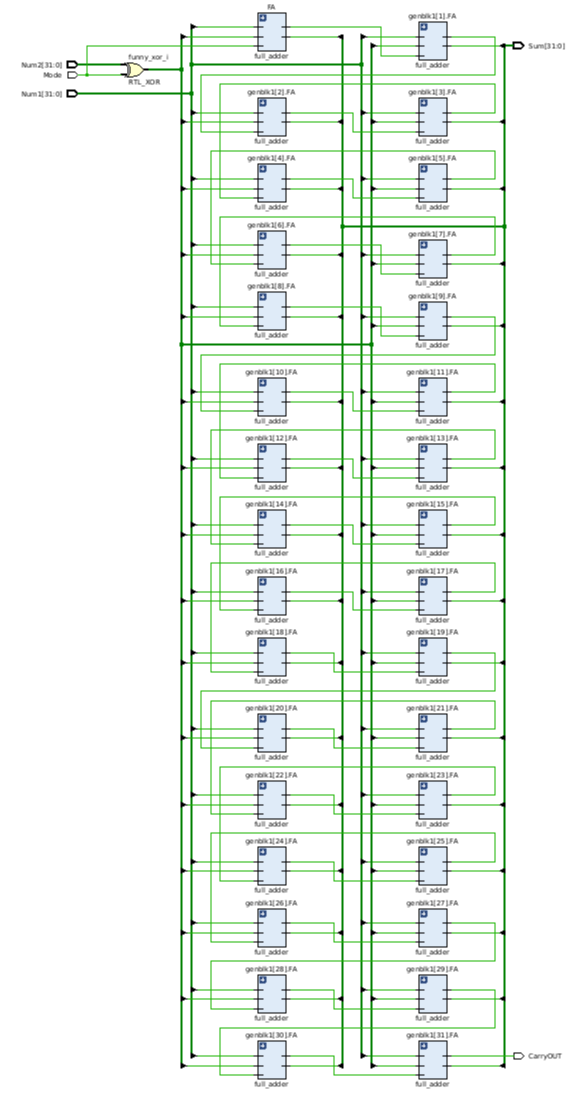
\includegraphics[width=0.5\textwidth]{part-4-schem.png}
    \label{32 Bit Adder/Subtractor}
\end{figure}

And when written up in verilog, has the following text:
\begin{lstlisting}[label={label}, style=Verilog]
module thirtytwo_bit_multi_adder( // part 4
    input[31:0] Num1, Num2,
    input Mode, // carryIN is the mode for reference
    output[31:0] Sum,
    output CarryOUT
  );
  
  wire[31:0] funny_xor, carry;

  assign funny_xor = Num2 ^ {32{Mode}}; // xo's Num2 with the mode for 2's complement subtraction.
  
  genvar i;

  generate
    full_adder FA(.A(Num1[0]), .B(funny_xor[0]), .CarryIN(Mode), .Sum(Sum[0]), .CarryOUT(carry[0]));
    for (i = 1; i < 32; i = i + 1) begin
      full_adder FA(.A(Num1[i]), .B(funny_xor[i]), .CarryIN(carry[i - 1]), .Sum(Sum[i]), .CarryOUT(carry[i]));
    end
  endgenerate
  
  assign CarryOUT = carry[31];

endmodule
\end{lstlisting}

And when tested, used the following testbench:
\begin{lstlisting}[label={label}, style=Verilog]
module testbench_part4();
  reg[31:0] num1, num2;
  reg mode;
  
  wire [31:0] sum;
  wire carryout;
  
  // CarryIN is the mode (0 for addition; 1 for subtractions)
  thirtytwo_bit_multi_adder UUT(.Num1(num1), .Num2(num2), .Mode(mode), .CarryOUT(carryout), .Sum(sum));

  initial begin

    mode = 0;
    num1 = 32'd50;
    num2 = 32'd25;
    #10;

    mode = 1;
    num1 = 32'd50;
    num2 = 32'd25;
    #10;

  end

endmodule
\end{lstlisting}
\newpage
And, when simulated to confirm the addition, and subtraction, of 50 and 25, it gave out the following waveform:
\begin{figure}[!htbp]
    \centering
    \caption{Waveform Addition/Subtraction Waveform}
    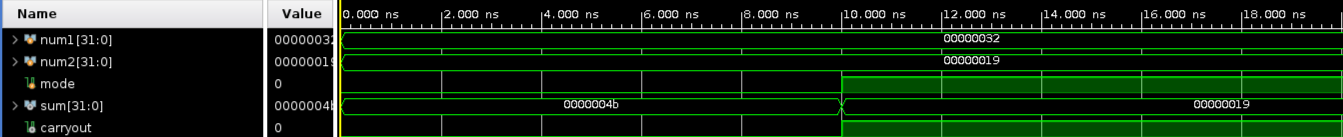
\includegraphics[width=1\textwidth]{part-4-waveform.png}
    \label{Waveform Part 4}
\end{figure}

And of which compiles to the followng truth table showing what the "Mode" change does to the number result:
\begin{center}
    Truth Table for 32 Bit Adder/Subtractor
    \begin{displaymath}
    \begin{array}{|c c c|c|}
      A & B & Mode & Result\\
    \hline
      50 & 25 & F & 75 \\
      50 & 25 & T & 25 \\
    \end{array}
    \end{displaymath}
\end{center}

Of which you can see, the "mode" simply switches the base addition of the decimal values of 50 and 25, to, when flicked to True/1, to being the subtraction of the second number to the first.\\

Now, while in this testcase example, we utilized a simple array of full-adders, we also could use an array of 4 Ripple Carry Adders (as those are more optimized for power and therefore area costs, unlike latency), and would therefore be superior to the schematic and code above, at least for the goals of the assignment given. Alongside this, at least with the current design that I've described in verilog above, it is a happy medium between all modes due to the fact that it is the simplest form of how one could make a 32 bit adder, of which is just a sequential chain of adders feeding into one another their carryINs and carryOUTs. And, yes, while there is latency involved, it would also, at least, provide its purpose as a general run of the mill 32-bit adder/subtractor.
\newpage



\section{Conclusion}
Now, in conclusion, we have learned the following things, listed of course in paragraph order in chronological order of this report.\\

First we learned on how to make a full adder, of which takes in 2 half adders, of which comprise of 2 gates (one AND and one XOR), and have an additional OR making it a total of 5 gates total per full adder.\\

Secondly, we learned that there are tradeoffs to how we design digital systems as a computer hardware engineer. Of which are specifically the timing of the system (also known as latency of the calculation), the area/size of the actual hardware proper, the performance/speed of the hardware (as well as if it is running in parallel or sequential), and finally the power it consumes as a component. Alongside this, we learned of 2 types of scalable multi-bit adders: the Ripple Carry Adder, and the Carry Look-Ahead Adder. Of which have the following pro's and con's:\\

The Ripple Carry Adder has the pro that it's simple to make and use, as well as uses less area and power compared to the Carry Look-Ahead Adder. It, however, loses out in its speed as well as timing, due to the fact that every bit in the addition requires the computation of the bit before it before it can continue, meaning that as you scale to 32 bits or even 64, significant delays occur.\\

For Carry Look-Ahead Adders, it is more performance and timing efficient than standard adder chains, and even the Ripple Carry Adder, BUT has a problem in that it is much more complex, as well as takes up much more power due to that complexity (due to its 56 gates compared to the Ripple Carry Adder's 40 gates), alongside its area impact, making it useful only for large scale additions and subtractions, that must be completed as fast as possible.\\

\end{document}
